\subsection{Getränkeschlitten}
\label{subsec:Getränkeschlitten}

Um ein Getränk möglichst ruckelfrei und stabil von einem zum anderen Punkt befördern zu können wurde auf ein Schlittensystem zurückgegriffen, welches so ähnlich auch im 3D-Druck Bereich eingesetzt wird. Dieses besteht ebenfalls aus einem X-Profil gemäss Kapitel \ref{subsec:Rahmen}, einem Schlitten, einem Riemen, einem Riemenspanner und einem Zahnrad. 

\begin{figure}[H]
	\centering
	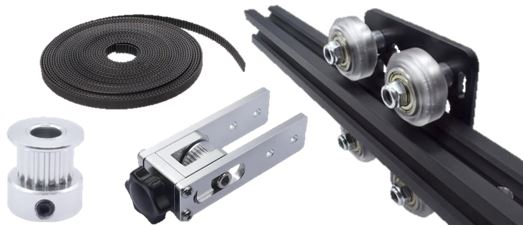
\includegraphics[width=0.6\textwidth]{graphics/Schlitten}
	\caption{Bauteile für den Schlitten des Partymixers \cite{shop4649026_store_2020_nodate} \cite{super_3d_technology_co_limited_2020_nodate} \cite{super_3d_technology_co_limited_1set_nodate} \cite{super_3d_technology_co_limited_2gtgt2_nodate}}
	\label{fig:Schlitten}
\end{figure}

Der Schlitten verfügt über zwei fest angebrachte Rollen auf der einen Seite und über zwei verstellbare Rollen auf der anderen Seite des Profils. Dies ermöglicht eine saubere Zentrierung des Schlittens. Der Riemen wird innerhalb des Profils geführt, was einerseits den Riemen schützt und anderseits einen schöneren Optik dient. Am einen Ende des X-Profils befindet sich der Riemenspanner, mit welchem sich die Spannung des Riemens einstellen lässt und am anderen Ende das Zahnrad, welches vom Motor angetrieben wird. 

Um den Motor und den Encoder montieren zu können, wurde eine Halterung entworfen und im 3D-Drucker ausgedruckt. Da die Achse des Motors relativ kurz ist und das Zahnrad sich in einem grösseren Abstand zum Montageort des Motors befindet, wurde eine Achse aus Aluminium auf der Drehbank gedreht.  Damit keine Flüssigkeit in das Profil rein tropft, wurde der Schlitten nicht direkt unter den Pumpen installiert, sondern ein wenig versetzt. Um das Glas jedoch trotzdem mittig unter den Pumpen führen zu können, wurde eine Glasauflage im 3D-Drucker gedruckt, welche auch den Riemen sauber im Profil führt. Diese Teile sind in Abbildung \ref{fig:Motorhalterung} zu sehen.    

\begin{figure}[H]
	\centering
	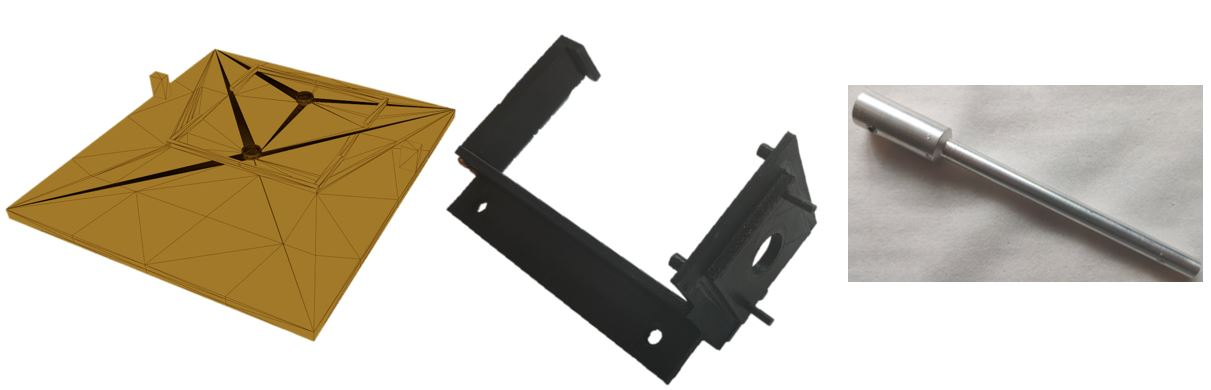
\includegraphics[width=0.9\textwidth]{graphics/Motorhalterung}
	\caption{Schlitten, Motorhalterung und Achse des PartyMixers}.
	\label{fig:Motorhalterung}
\end{figure} 